\chapter{Assembly and Dynamics of Rod-Shaped Colloids}
\section{Introduction}

\tempfigure{Colloidal rod examples}
\begin{itemize}
\statement{Natural rod systems}
\statement{Systems studied by Solomon}
\statement{Janus colloids: Granick}
\statement{Interest in Janus rods}
\end{itemize}

\section{Experimental Procedure}
\subsection{Stop-Flow Lithography}

\tempfigure{Photo of SFL setup; SFL flowchart; example experiment}
\begin{itemize}
\done{Microscope setup}
\done{Pressure system--Rob}
\done{LabView controller for SFL}
\done{Design of microfluidic devices for up to 3-stream SFL}
\done{Fabrication of microfluidic devices}
\end{itemize}

\tempfigure{Examples of SFL masks used in rod experiments}
\subsection{Mask Design}
\begin{itemize}
\done{Demagnification using 60X objective}
\done{Design parameters}
\done{Rod aspect ratios used}
\end{itemize}

\subsection{Particle Collection}
\begin{itemize}
\done{Considerations for collection}
\done{Solvents used}
\done{Pipettes}
\done{Fluorosilane coatings}
\end{itemize}

\subsection{Diffusion Measurements}
\begin{itemize}
\done{Confocal microscopy setup}
\done{Space and time resolution requirements}
\done{Fluorescence requirements}
\end{itemize}

\section{Results and Discussion}

\tempfigure{Resolution test mask; image of resulting particles}
\subsection{Resolution}
\begin{itemize}
\done{Limiting factors for SFL resolution: mask design, optics, flow effects}
\notdone{Resolution limits constrained by 60X lens--need to redo this (~1 hour work)}
\done{Resolution limits for Janus rods--interface effects}
\end{itemize}

\tempfigure{Image of rod tracking}
\tempfigure{Plots of translational and rotational diffusion data}
\subsection{Translational and Rotational Diffusion}
\begin{itemize}
\done{Particle collection--PEGDA vs TMPTA}
\done{Compare particle/solvent/surface effects}
\notdone{2D diffusion size series: TMPTA in toluene (additional experiments may be required)}
\notdone{Analyze diffusion data for rods (partially done).}
\end{itemize}

\tempfigure{Show fabricated Janus rods of various sizes.}
\tempfigure{Assembly of rods in various solvents}

\begin{figure}
\begin{center}
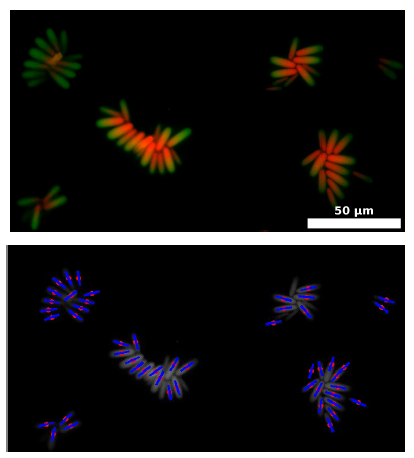
\includegraphics{figures/assembled-janus-tracked.png}
\end{center}
\caption{(a) Janus rods which have self-assembled into ordered 
clusters are identified and separated, and (b) their 
positions and orientations are labeled.}
\label{fig:assembled-janus-tracking}
\end{figure}

\subsection{Self-Assembly of Janus Rods}
\begin{itemize}
\done{Fabrication of Janus rods: various sizes (figure)}
\done{Comparison of self-assembly in various solvents (figure)}
\done{Small clusters vs large structures}
\done{Alignment of assembled rods}
\done{Image segmentation for analyzing structures}
\notdone{Some more good-looking images may be required}
\end{itemize}